\documentclass{article}
% === includs ====
\usepackage{import}
\import{envs/}{answer}
\import{envs/}{Terminal}

\usepackage{hyperref}
\usepackage{tikz}
\usepackage{graphicx}
\usepackage[export]{adjustbox}
\usepackage{float}
\usepackage{fancyhdr}
\usepackage[font=small]{caption}
\usepackage{mathtools}
\usepackage{booktabs}
\usepackage{enumitem}
\usepackage{xcolor}
\usepackage{eso-pic}
\usepackage{xepersian} 
\usepackage{fontspec}
\usepackage{pgfplots}



\pgfplotsset{compat=1.18}
\usepgfplotslibrary{statistics}
\graphicspath{{./images}}
\setmonofont{Liberation Mono} 

% === Fonts ===
% Persian text font
\settextfont[
    Path = ./fonts/,
    Extension = .ttf,
    BoldFont = *-Bold,
    ItalicFont = *-Italic,
    Script = Arabic
]{BNazanin}

% Latin text font
\setlatintextfont[
    Path = ./fonts/,
    Extension = .ttf,
    BoldFont = *-Bold,
    ItalicFont = *-Italic,
    BoldItalicFont = *-BoldItalic
]{Times}


% === Page style ===
\pagestyle{fancy}
\fancyhf{} 
\rhead{\footnotesize مستندات پروژه درس مهندسی نرم‌افزار۲} 
\rfoot{\thepage} 
\renewcommand{\footrulewidth}{0.4pt}
\renewcommand{\labelenumi}{\alph{enumi})}
\usetikzlibrary{arrows.meta}
\fancypagestyle{p4}{\fancyfoot[L]{\latinfont \beginL \footnotesize 1-Learning Rate }}




% === Document ===
\begin{document}
  \thispagestyle{empty}
  \vspace*{-3cm}
  \begin{center}
      \fontsize{40}{50}\selectfont به نام خدا\\[2cm]

      
\includegraphics[height=.3\textheight, width=.55\textwidth]{images/AUTlogo.png}\\[0.5cm]
      \Huge\textbf{دانشکده مهندسی \\ کامپیوتر و فناوری اطلاعات}\\[1cm]
      {\Huge \textbf{مستندات پروژه درس مهندسی نرم‌افزار۲} \\[1.5cm]}
      {\huge کاوه احمدی ۴۰۱۳۱۹۰۴}\\
      {\huge آرمینا متقی ۴۰۱۳۱۴۱۸}\\[0.5cm]
      {\huge تیر ۱۴۰۵} 
  \end{center}
\newpage
\section{\lr{Product Vision}}

پلتفرم \lr{End-to-End Ticketing} یک سیستم با \lr{High Availability} برای مدیریت \lr{Flash Sales} و ترافیک بالا است. هدف سیستم جلوگیری از \lr{Downtime} و مقیاس‌پذیری پویا برای توسعه سیستم است.

\subsection{کاربران هدف}

\begin{description}[font=$\bullet$~\normalsize\scshape]
\item \lr{End-User} نیازمند جستجوی سریع رویداد، مشاهده نقشه \lr{Real-Time} سالن، قرارگیری در \lr{Virtual Waiting Room} و دریافت \lr{QR Code}.
\item \lr{Admin} نیازمند طراحی سالن چندبخشی، تنظیم \lr{Dynamic Pricing} و مشاهده \lr{Dashboards} تحلیلی در لحظه.
\end{description}

\subsection{معیارهای کلیدی عملکرد}

\begin{enumerate}
\item \lr{Checkout Completion Rate} بررسی درصد موفقیت پرداخت پس از قفل صندلی.
\item \lr{Seat Lock Expiration Rate} بررسی نرخ انقضای قفل‌های موقت \lr{Redis}.
\item \lr{Latency} حفظ زمان پاسخگویی زیر یک ثانیه و پایداری \lr{Uptime} بالا.
\item \lr{Gross Merchandise Value} پیگیری درآمدزایی سیستم به صورت زنده.
\end{enumerate}

\vspace{1cm}

\section{\lr{Risk Mitigation Analysis}}

\subsection{ریسک اول \lr{Flash Traffic Spikes}}

شرح ریسک: هجوم همزمان ربات‌ها و کاربران به \lr{API Gateway} و خطر از کار افتادن \lr{Event Catalog}.

راهکار مهندسی:

\begin{description}[font=$\bullet$~\normalsize\scshape]
\item اجرای \lr{Virtual Waiting Room} برای \lr{Traffic Throttling}.
\item تنظیم \lr{Rate Limiting} در لایه \lr{Edge}.
\item استفاده از \lr{Auto-scaling} در \lr{Kubernetes}.
\end{description}

\subsection{ریسک دوم \lr{Race Conditions}}

شرح ریسک: درخواست همزمان برای یک صندلی و خطر \lr{Double-Booking}.

راهکار مهندسی:

\begin{description}[font=$\bullet$~\normalsize\scshape]
\item پیاده‌سازی \lr{Distributed Locks} توسط \lr{Redis} با \lr{Time-To-Live} مشخص.
\item استفاده از \lr{Optimistic Concurrency Control} در \lr{PostgreSQL}.
\end{description}

\subsection{ریسک سوم \lr{Payment Gateway Timeout}}

شرح ریسک: قطعی درگاه بانکی در حین \lr{Checkout} و گیر کردن صندلی در حالت رزرو.

راهکار مهندسی:

\begin{description}[font=$\bullet$~\normalsize\scshape]
\item اجرای \lr{Saga Pattern} و تراکنش‌های \lr{Compensation}.
\item آزادسازی خودکار قفل‌ها و بازگشت صندلی به سیستم در صورت دریافت خطا.
\end{description}

\subsection{ریسک چهارم \lr{Network Partitioning}}

شرح ریسک: قطعی ارتباط بین سرویس‌ها مانند عدم ارسال \lr{SMS} تایید به مشتری.

راهکار مهندسی:

\begin{description}[font=$\bullet$~\normalsize\scshape]
\item استفاده از \lr{Asynchronous Messaging} توسط \lr{Message Brokers}.
\item ارسال پیام‌های ناموفق به \lr{Dead-Letter Queue} جهت تلاش مجدد.
\end{description}

\section{\lr{Product Vision}}

پلتفرم \lr{End-to-End Ticketing} یک سیستم با \lr{High Availability} برای مدیریت \lr{Flash Sales} و ترافیک بالا است. هدف سیستم جلوگیری از \lr{Downtime} و مقیاس‌پذیری پویا برای توسعه سیستم است.

\subsection{کاربران هدف}

\begin{description}[font=$\bullet$~\normalsize\scshape]
\item \lr{End-User} نیازمند جستجوی سریع رویداد مشاهده نقشه \lr{Real-Time} سالن قرارگیری در \lr{Virtual Waiting Room} و دریافت \lr{QR Code}.
\item \lr{Admin} نیازمند طراحی سالن چندبخشی تنظیم \lr{Dynamic Pricing} و مشاهده \lr{Dashboards} تحلیلی در لحظه.
\end{description}

\subsection{معیارهای کلیدی عملکرد}

\begin{enumerate}
\item \lr{Checkout Completion Rate} بررسی درصد موفقیت پرداخت پس از قفل صندلی.
\item \lr{Seat Lock Expiration Rate} بررسی نرخ انقضای قفل‌های موقت \lr{Redis}.
\item \lr{Latency} حفظ زمان پاسخگویی زیر یک ثانیه و پایداری \lr{Uptime} بالا.
\item \lr{Gross Merchandise Value} پیگیری درآمدزایی سیستم به صورت زنده.
\end{enumerate}

\vspace{1cm}

\section{\lr{Risk Mitigation Analysis}}

\subsection{ریسک اول \lr{Flash Traffic Spikes}}

شرح ریسک هجوم همزمان ربات‌ها و کاربران به \lr{API Gateway} و خطر از کار افتادن \lr{Event Catalog}.

راهکار مهندسی

\begin{description}[font=$\bullet$~\normalsize\scshape]
\item اجرای \lr{Virtual Waiting Room} برای \lr{Traffic Throttling}.
\item تنظیم \lr{Rate Limiting} در لایه \lr{Edge}.
\item استفاده از \lr{Auto-scaling} در \lr{Kubernetes}.
\end{description}

\subsection{ریسک دوم \lr{Race Conditions}}

شرح ریسک درخواست همزمان برای یک صندلی و خطر \lr{Double-Booking}.

راهکار مهندسی

\begin{description}[font=$\bullet$~\normalsize\scshape]
\item پیاده‌سازی \lr{Distributed Locks} توسط \lr{Redis} با \lr{Time-To-Live} مشخص.
\item استفاده از \lr{Optimistic Concurrency Control} در \lr{PostgreSQL}.
\end{description}

\subsection{ریسک سوم \lr{Payment Gateway Timeout}}

شرح ریسک قطعی درگاه بانکی در حین \lr{Checkout} و گیر کردن صندلی در حالت رزرو.

راهکار مهندسی

\begin{description}[font=$\bullet$~\normalsize\scshape]
\item اجرای \lr{Saga Pattern} و تراکنش‌های \lr{Compensation}.
\item آزادسازی خودکار قفل‌ها و بازگشت صندلی به سیستم در صورت دریافت خطا.
\end{description}

\subsection{ریسک چهارم \lr{Network Partitioning}}

شرح ریسک قطعی ارتباط بین سرویس‌ها مانند عدم ارسال \lr{SMS} تایید به مشتری.

راهکار مهندسی

\begin{description}[font=$\bullet$~\normalsize\scshape]
\item استفاده از \lr{Asynchronous Messaging} توسط \lr{Message Brokers}.
\item ارسال پیام‌های ناموفق به \lr{Dead-Letter Queue} جهت تلاش مجدد.
\end{description}

\vspace{1cm}

\section{\lr{Diagrams}}

\subsection{\lr{Use Case Diagram}}

این بخش شامل \lr{Use Case Diagram} سیستم است که تعامل بین \lr{Actors} و \lr{Use Cases} را نشان می‌دهد.

\begin{figure}[h]
\centering
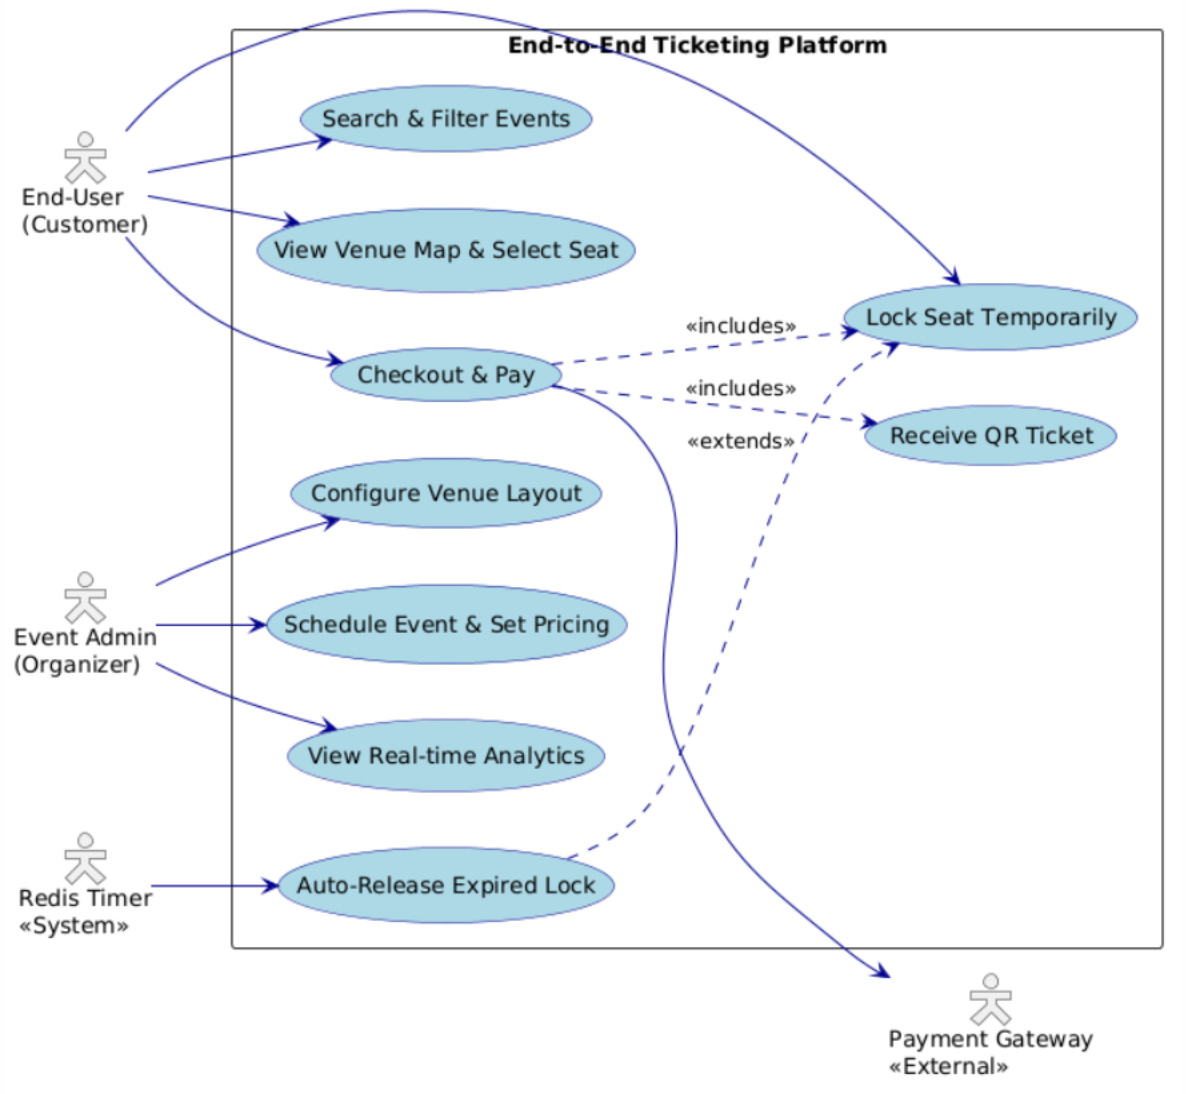
\includegraphics[width=0.9\textwidth]{usecase.png}
\end{figure}

\subsubsection{تحلیل اکترها}

\begin{description}[font=$\bullet$~\normalsize\scshape]
\item \lr{End-User} خریدار بلیت که عملیاتی مانند جستجو انتخاب صندلی و \lr{Checkout} را انجام می‌دهد.
\item \lr{Event Admin} مدیر سیستم که وظیفه \lr{Configure Venue Layout} و بررسی \lr{Analytics} را بر عهده دارد.
\item \lr{Payment Gateway} یک \lr{External Actor} برای پردازش تراکنش‌های مالی.
\item \lr{Redis Timer} یک \lr{System Actor} برای مدیریت زمان انقضای قفل صندلی‌ها.
\end{description}

\subsubsection{تحلیل روابط}

\begin{description}[font=$\bullet$~\normalsize\scshape]
\item \lr{Includes} کاربر برای تکمیل \lr{Checkout} حتما باید مرحله \lr{Lock Seat Temporarily} را انجام دهد.
\item \lr{Extends} در صورت عدم پرداخت در زمان مقرر سیستم به صورت خودکار \lr{Auto-Release Expired Lock} را اجرا می‌کند تا صندلی آزاد شود.
\end{description}

\subsection{\lr{Sequence Diagram}}

این بخش \lr{Sequence Diagram} فرآیند رزرو و پرداخت بلیت را نشان می‌دهد که تعامل بین کامپوننت‌ها را در طول زمان مشخص می‌کند.

\begin{figure}[h]
\centering
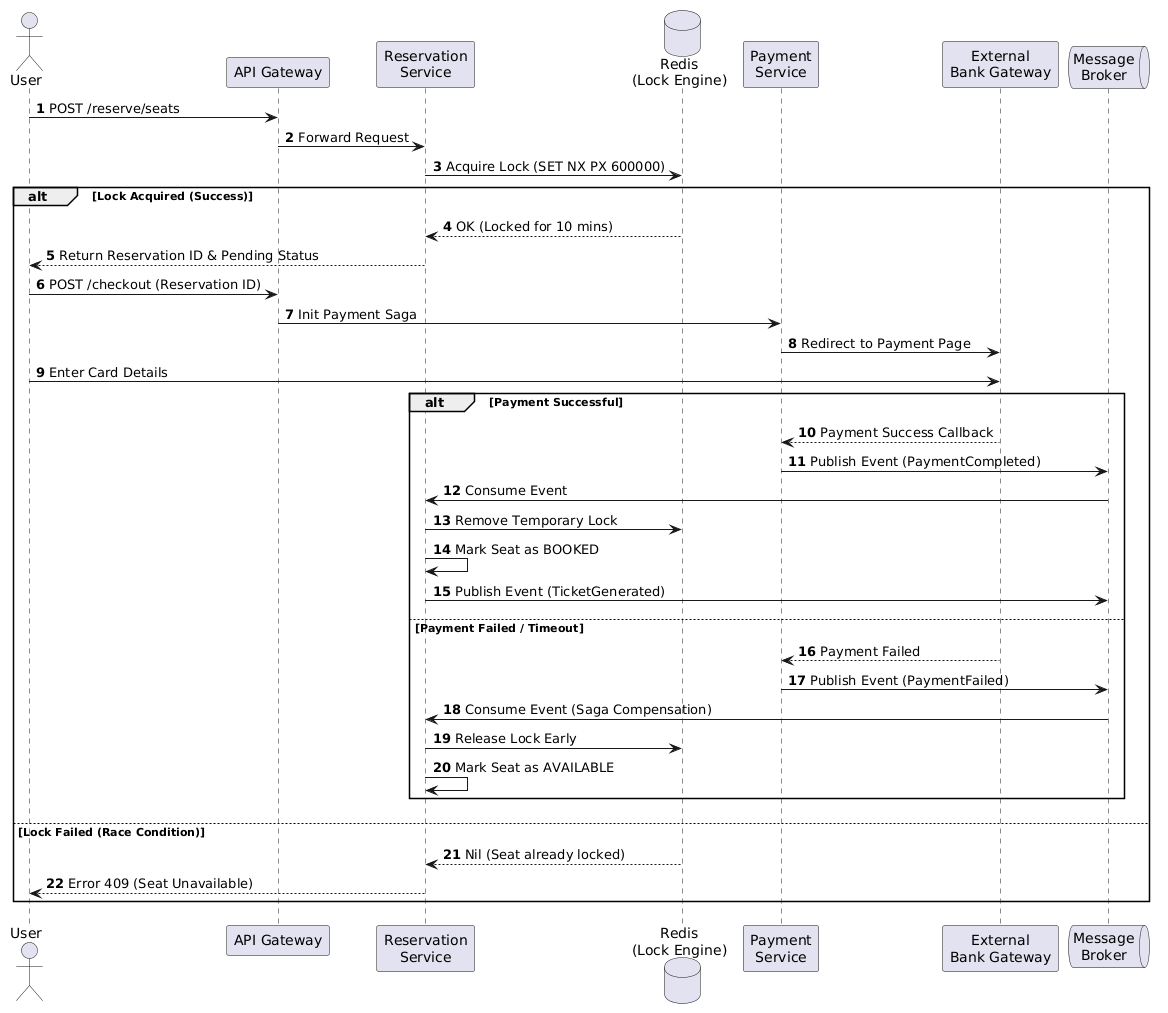
\includegraphics[width=0.9\textwidth]{sequence.png}
\end{figure}

\subsubsection{تحلیل جریان اصلی}

\begin{description}[font=$\bullet$~\normalsize\scshape]
\item \lr{Lock Acquisition} کاربر درخواست \lr{POST /reserve/seats} را ارسال می‌کند و \lr{Reservation Service} با دستور \lr{SET NX PX 600000} صندلی را در \lr{Redis} برای ده دقیقه قفل می‌کند.
\item \lr{Payment Saga} پس از دریافت \lr{Reservation ID} کاربر عملیات \lr{Checkout} را آغاز کرده و به صفحه پرداخت هدایت می‌شود.
\end{description}

\subsubsection{تحلیل سناریوها}

\begin{description}[font=$\bullet$~\normalsize\scshape]
\item \lr{Payment Successful} پس از \lr{Callback} موفق \lr{Payment Service} رویداد \lr{PaymentCompleted} را منتشر می‌کند سپس قفل موقت حذف شده و صندلی به وضعیت \lr{BOOKED} تغییر می‌کند و رویداد \lr{TicketGenerated} منتشر می‌شود.
\item \lr{Payment Failed} در صورت شکست یا \lr{Timeout} رویداد \lr{PaymentFailed} منتشر شده و \lr{Saga Compensation} اجرا می‌شود تا قفل زودتر آزاد و صندلی به وضعیت \lr{AVAILABLE} برگردد.
\item \lr{Race Condition} اگر صندلی از قبل قفل شده باشد \lr{Redis} مقدار \lr{Nil} برمی‌گرداند و سیستم خطای \lr{Error 409} را نمایش می‌دهد.
\end{description}


\subsection{\lr{Deployment Diagram}}

این بخش \lr{Deployment Diagram} است که نحوه استقرار کامپوننت‌ها بر روی زیرساخت فیزیکی و ابری را نمایش می‌دهد.

\begin{figure}[h]
\centering
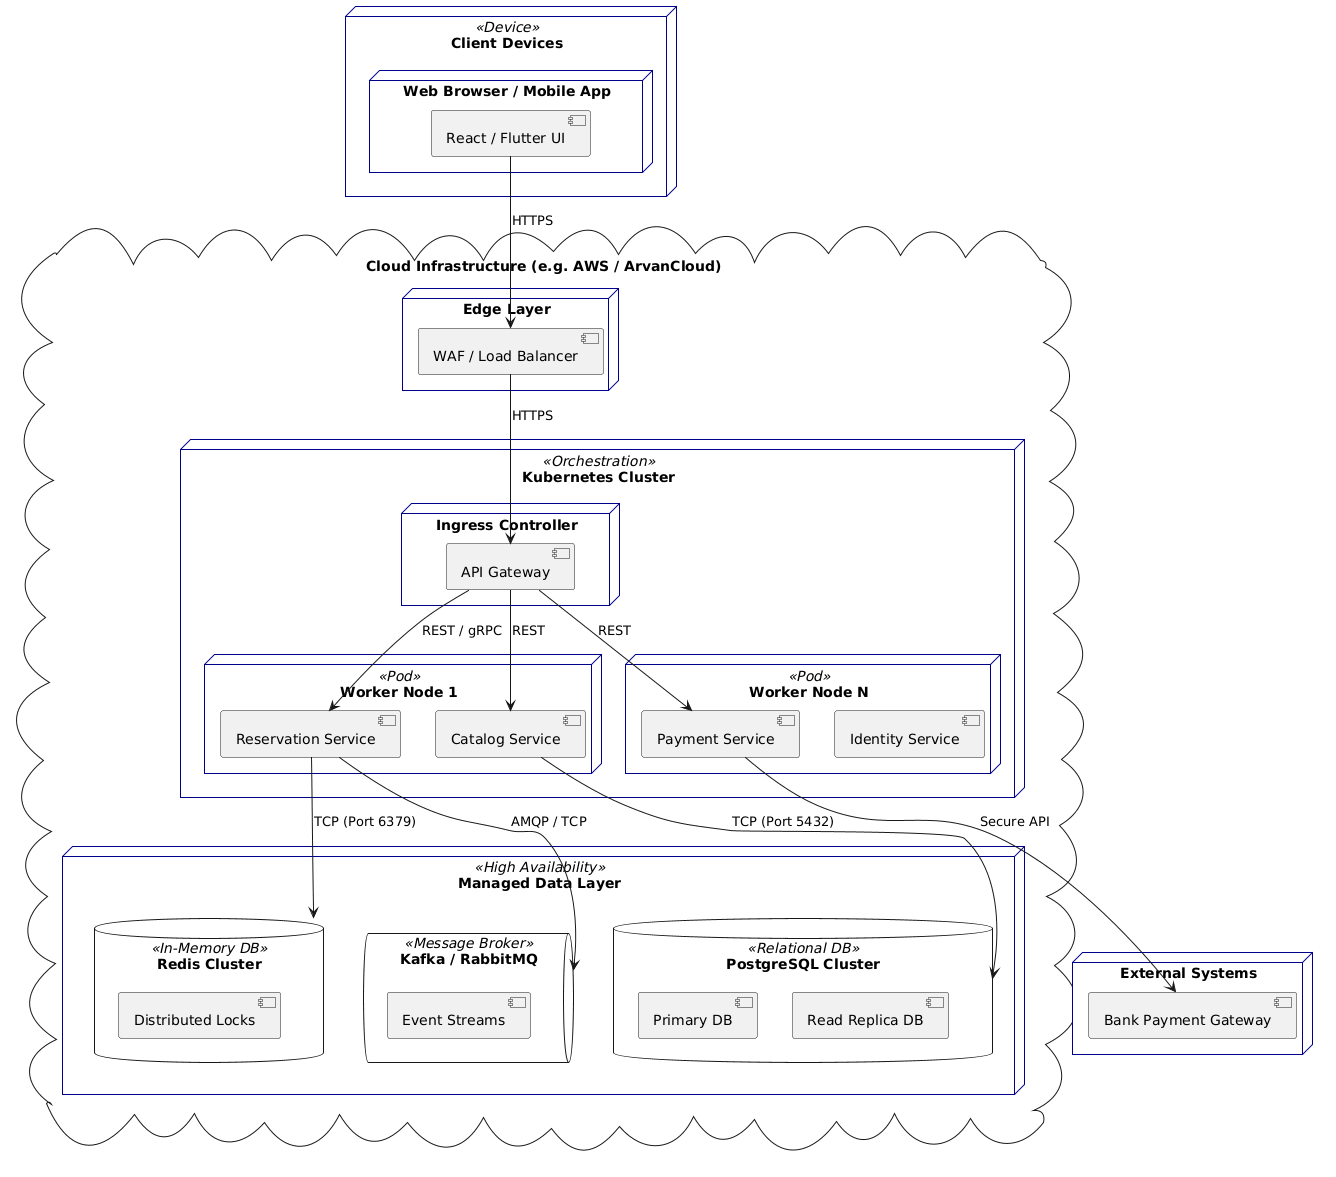
\includegraphics[width=0.9\textwidth]{deployment.png}
\end{figure}

\subsubsection{تحلیل لایه‌ها}

\begin{description}[font=$\bullet$~\normalsize\scshape]
\item \lr{Client Devices} شامل \lr{Web Browser} و \lr{Mobile App} است که با استفاده از \lr{React / Flutter UI} پیاده‌سازی شده و از طریق \lr{HTTPS} ارتباط برقرار می‌کند.
\item \lr{Edge Layer} شامل \lr{WAF / Load Balancer} برای مدیریت ترافیک ورودی و امنیت است.
\item \lr{Kubernetes Cluster} یک لایه \lr{Orchestration} که شامل \lr{Ingress Controller} و \lr{Worker Node} های مختلف برای اجرای سرویس‌ها است.
\item \lr{Managed Data Layer} با قابلیت \lr{High Availability} شامل \lr{Redis Cluster} و \lr{Kafka / RabbitMQ} و \lr{PostgreSQL Cluster} است.
\end{description}

\subsubsection{تحلیل ارتباطات}

\begin{description}[font=$\bullet$~\normalsize\scshape]
\item \lr{Redis Connection} سرویس‌ها از طریق \lr{TCP Port 6379} به \lr{Distributed Locks} دسترسی دارند.
\item \lr{Database Connection} ارتباط با \lr{PostgreSQL} از طریق \lr{TCP Port 5432} انجام می‌شود.
\item \lr{External API} پرداخت‌ها از طریق \lr{Secure API} به \lr{Bank Payment Gateway} متصل می‌شوند.
\end{description}


\subsection{\lr{Component Diagram}}

این بخش \lr{Component Diagram} است که کامپوننت‌های اصلی سیستم و ارتباط بین \lr{Microservices} را در قالب \lr{Bounded Contexts} نشان می‌دهد.

\begin{figure}[h]
\centering
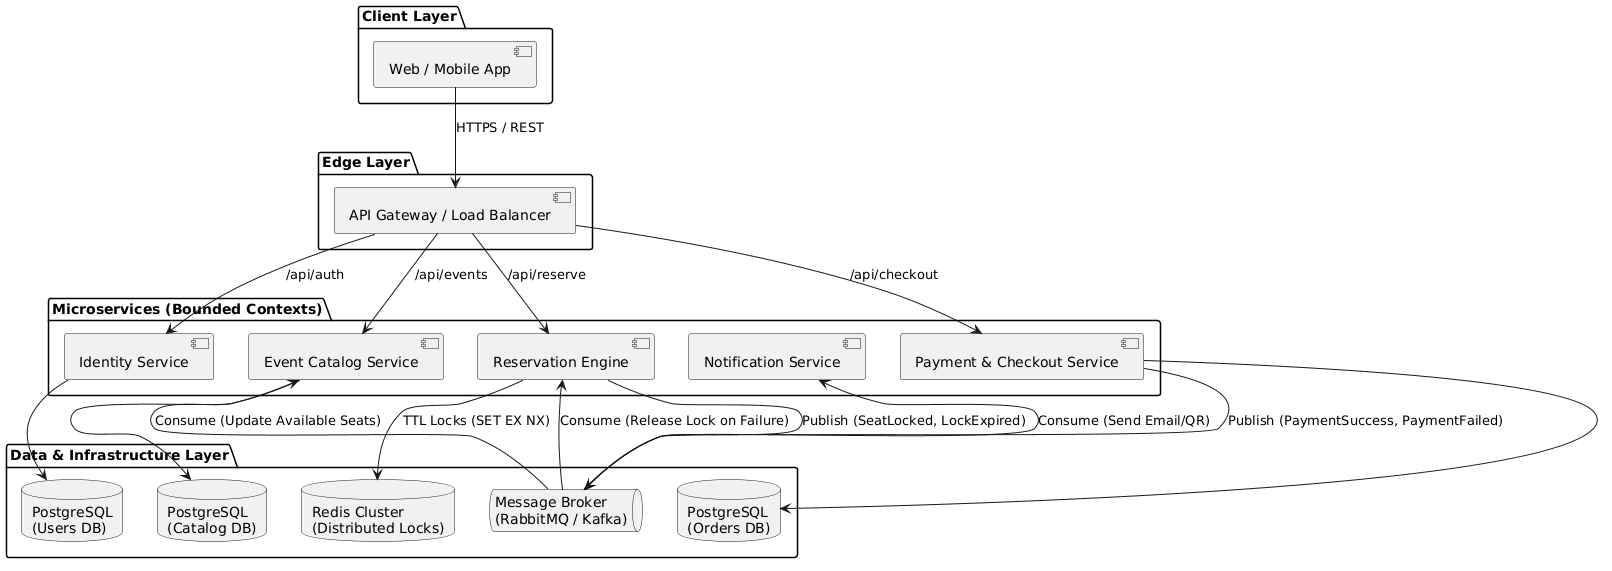
\includegraphics[width=0.9\textwidth]{component.png}
\end{figure}

\subsubsection{تحلیل لایه‌ها}

\begin{description}[font=$\bullet$~\normalsize\scshape]
\item \lr{Client Layer} شامل \lr{Web / Mobile App} است که از طریق \lr{HTTPS / REST} با سیستم ارتباط برقرار می‌کند.
\item \lr{Edge Layer} شامل \lr{API Gateway / Load Balancer} است که درخواست‌ها را به سرویس‌های مربوطه هدایت می‌کند.
\item \lr{Microservices} شامل \lr{Identity Service} و \lr{Event Catalog Service} و \lr{Reservation Engine} و \lr{Notification Service} و \lr{Payment \& Checkout Service} است.
\item \lr{Data \& Infrastructure Layer} شامل چند \lr{PostgreSQL} مجزا و \lr{Redis Cluster} و \lr{Message Broker} است.
\end{description}

\subsubsection{تحلیل تعاملات رویدادمحور}

\begin{description}[font=$\bullet$~\normalsize\scshape]
\item \lr{Distributed Locks} موتور رزرو از \lr{TTL Locks} با دستور \lr{SET EX NX} در \lr{Redis} استفاده می‌کند.
\item \lr{Event Publishing} رویدادهای \lr{SeatLocked} و \lr{LockExpired} و \lr{PaymentSuccess} و \lr{PaymentFailed} از طریق \lr{Message Broker} منتشر می‌شوند.
\item \lr{Event Consuming} سرویس‌ها رویدادها را برای \lr{Update Available Seats} و \lr{Release Lock on Failure} و \lr{Send Email/QR} مصرف می‌کنند.
\end{description}


\subsection{\lr{Class Diagram}}

این بخش \lr{Class Diagram} است که ساختار کلاس‌ها و روابط بین موجودیت‌های اصلی سیستم را نمایش می‌دهد.

\begin{figure}[h]
\centering
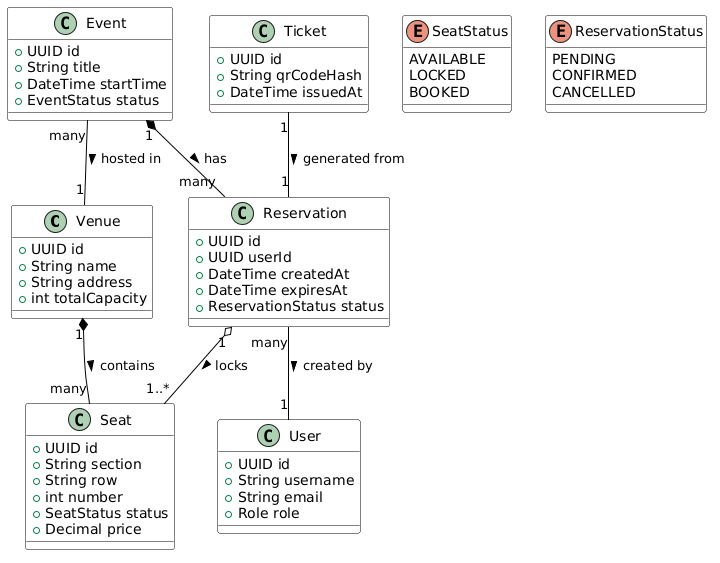
\includegraphics[width=0.7\textwidth]{class.png}
\end{figure}

\subsubsection{تحلیل کلاس‌ها}

\begin{description}[font=$\bullet$~\normalsize\scshape]
\item \lr{Event} رویداد اصلی که شامل \lr{title} و \lr{startTime} و \lr{status} است و در یک \lr{Venue} برگزار می‌شود.
\item \lr{Venue} محل برگزاری که شامل \lr{name} و \lr{address} و \lr{totalCapacity} است و شامل چندین \lr{Seat} می‌باشد.
\item \lr{Reservation} رزرو که با \lr{userId} و \lr{createdAt} و \lr{expiresAt} مشخص می‌شود و صندلی‌ها را قفل می‌کند.
\item \lr{Ticket} بلیت نهایی که شامل \lr{qrCodeHash} است و از یک \lr{Reservation} تولید می‌شود.
\item \lr{Seat} صندلی که شامل \lr{section} و \lr{row} و \lr{number} و \lr{price} است.
\item \lr{User} کاربر که شامل \lr{username} و \lr{email} و \lr{role} است.
\end{description}

\subsubsection{تحلیل \lr{Enumerations}}

\begin{description}[font=$\bullet$~\normalsize\scshape]
\item \lr{SeatStatus} شامل مقادیر \lr{AVAILABLE} و \lr{LOCKED} و \lr{BOOKED} است.
\item \lr{ReservationStatus} شامل مقادیر \lr{PENDING} و \lr{CONFIRMED} و \lr{CANCELLED} است.
\end{description}


\subsection{\lr{Activity Diagram}}

این بخش \lr{Activity Diagram} است که جریان کاری فرآیند رزرو صندلی و پرداخت را همراه با شاخه‌های تصمیم‌گیری نشان می‌دهد.

\begin{figure}[h]
\centering
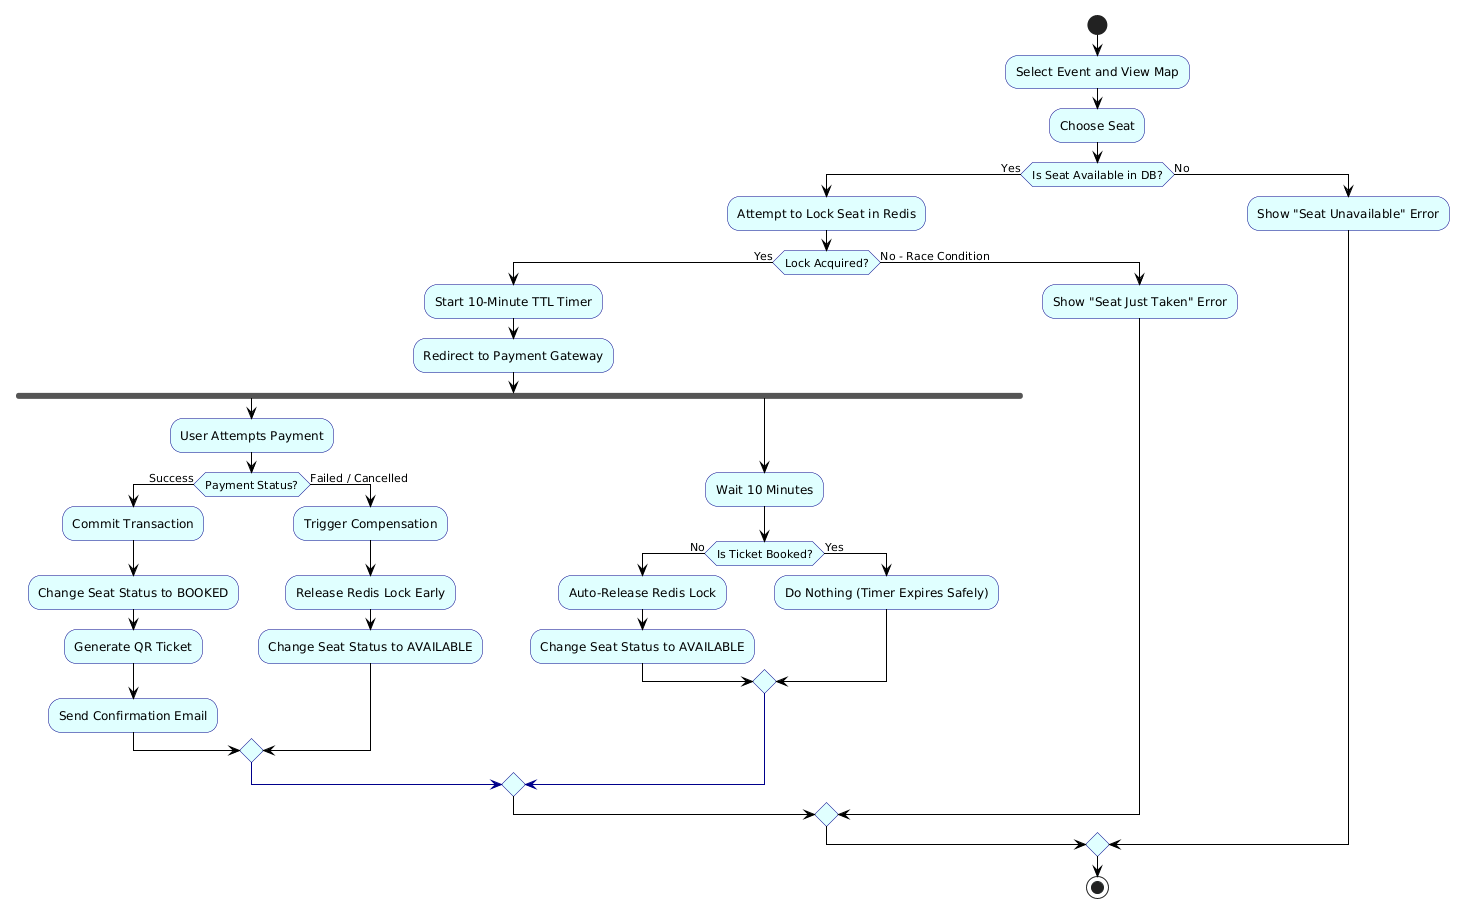
\includegraphics[width=0.9\textwidth]{activity.png}
\end{figure}

\subsubsection{تحلیل جریان انتخاب صندلی}

\begin{description}[font=$\bullet$~\normalsize\scshape]
\item \lr{Seat Availability} پس از \lr{Choose Seat} سیستم بررسی می‌کند که آیا صندلی در پایگاه‌داده موجود است در غیر این صورت خطای \lr{Seat Unavailable} نمایش داده می‌شود.
\item \lr{Lock Attempt} در صورت موجود بودن سیستم تلاش می‌کند صندلی را در \lr{Redis} قفل کند و اگر \lr{Race Condition} رخ دهد خطای \lr{Seat Just Taken} نمایش داده می‌شود.
\item \lr{TTL Timer} پس از قفل موفق یک تایمر ده دقیقه‌ای شروع شده و کاربر به \lr{Payment Gateway} هدایت می‌شود.
\end{description}

\subsubsection{تحلیل جریان پرداخت}

\begin{description}[font=$\bullet$~\normalsize\scshape]
\item \lr{Payment Success} در صورت موفقیت تراکنش \lr{Commit} شده و صندلی به \lr{BOOKED} تغییر می‌کند سپس \lr{QR Ticket} تولید و ایمیل تأیید ارسال می‌شود.
\item \lr{Payment Failed} در صورت شکست یا لغو \lr{Compensation} فعال شده و قفل زودتر آزاد و صندلی به \lr{AVAILABLE} برمی‌گردد.
\item \lr{Timeout Handling} در صورت گذشت ده دقیقه اگر بلیت \lr{Booked} نشده باشد قفل \lr{Redis} به صورت خودکار آزاد می‌شود در غیر این صورت تایمر بدون تأثیر منقضی می‌شود.
\end{description}

\end{document}
